\documentclass[11pt,letterpaper]{article}
\usepackage{hyperref}
\usepackage[spanish]{babel}
\usepackage{multirow} 
\usepackage{multicol} 
\usepackage{subfig}
\usepackage{amsmath} % for \text{}
\usepackage{gensymb}
\usepackage{float}
\usepackage{mathrsfs} 
\usepackage{minted}
\usepackage{hyperref}

\usepackage[utf8]{inputenc}
% Control de color en tablas muy versátil.
\usepackage[table]{xcolor}
 % LaTeX


\title{Plantilla Informe}
  
% $Rev: 5 $
% PAQUETES %%%%%%%%%%%%%%%%%%%%%%%%%%%%%%%%%%%%%%%%%%%%%%%%%%%%%%%%%%%%%%%%%%%%
\usepackage{graphicx}
\usepackage{listings}
\usepackage{xcolor}
\usepackage{multicol}
\usepackage{anysize} %Permitir distintas medidas de margenes
\usepackage{framed}
\usepackage{fancyhdr}
\usepackage[spanish]{babel}
\usepackage[utf8]{inputenc}

\fancyhf{} 
\chead{ Proyecto de T\'itulo I \vspace{0.3cm}}
\lhead{
\includegraphics[scale=0.1]{Log.png}}
\rfoot{\thepage}

\renewcommand{\footrulewidth}{0.25pt}

\addtolength{\headheight}{1.4cm}

% CONFIGURACION DE LISTINGS %%%%%%%%%%%%%%%%%%%%%%%%%%%%%%%%%%%%%%%%%%%%%%%%%%%
\newcommand{\AddUserKeywords}[1]{\lstset{morekeywords=[2]{#1}}}
\newcommand{\CodeSize}[1]{\lstset{basicstyle=#1\ttfamily}}
\newcommand{\CommentColor}{\color{green!60!black}}
\newcommand{\StringColor}{\color{red!70!black}}
\newcommand{\UserKeywordsColor}{\color{cyan!50!black}}
\newcommand{\KeywordsColor}{\color{blue}}

\lstdefinelanguage{CSharp}
{
	basicstyle=\small\ttfamily,
	keywordstyle=\KeywordsColor\textbf,
	keywordstyle=[2]\UserKeywordsColor,
	keywordstyle=[3]\StringColor,
	tabsize=2,
	morekeywords={abstract, as, base, bool, break, byte, case, 
		catch, char, checked,class, const, continue, decimal, 
		default, delegate, do, double, else, enum, event, explicit,
		extern, false, finally, fixed, float, for, foreach, get, goto, 
		if, implicit, in, int, interface, internal, is, lock, long,
		namespace, new, null, object, operator, out, override, 
		params, partial, private, protected, public, readonly, ref, return, 
		sbyte, sealed, set, short, sizeof, stackalloc, static, string,
		struct, switch, this, throw, try, typeof, true, uint, ulong, 
		unchecked, unsafe, ushort, using, value, virtual, volatile,
		void, while, where},
	morekeywords=[2]{Main,Console,String},
	morekeywords=[3]{@}, 
	commentstyle=\CommentColor,
	stringstyle=\StringColor,
	sensitive=true,
	morecomment=[l]{//},
	morecomment=[s]{/*}{*/},
	morestring=[b]",
	showstringspaces=false,
	aboveskip=0pt, 
	belowskip=0pt,
	mathescape=true
}

% Set as the default languaje
\lstset{language=CSharp}

\newcommand{\inguandesheader}{
	% Header Facultad Ingenieria Uandes			
	
\includegraphics[scale=0.5]{uandes.pdf}\hspace*{\fill}
}

\newcommand{\evaluationtitle}[2]{
	% T\'itulo
	\begin{center}
	\vspace{1ex}\Large #1\\
	\vspace{1ex}\small #2
	\end{center}
}


\newenvironment{guideexercise}[3]{
	\noindent\textbf{#1}	
	\vspace{-0.3cm}
	\begin{framed}
		\noindent\textsl{Dificultad:} #2\\
		\textsl{Etiquetas:} #3\\	
				
}{
	\end{framed}
	\vspace{0.3cm}
}

\renewcommand{\baselinestretch}{1.5}

\pagestyle{fancy}
\begin{document}

%% COMIENZO PORTADA-----------------------------------------

\begin{titlepage}

\begin{center}

\includegraphics[scale=0.3]{Log.png}\\
% Incrementamos el interlineado:
\vspace{1.0cm} {\LARGE Hito I\\ Ingenier\'ia Civil Industrial UANDES\\  Proyecto de T\'itulo I} \\

\vspace{1.5cm} \LARGE{Por:\\ Ezequiel Ortiz Torres \\ Gu\'ia: \\ Sebasti\'an Cea}

\vspace{2.3cm}

\vspace{.5cm} \today

\end{center}
\end{titlepage}

 %%%% FIN PORTADA ------------------------------------------

\tableofcontents
\newpage


\section{Introducci\'on}

Un proyecto con características medioambientales, sociales y gubernamentales es un proyecto ESG por sus siglas en inglés (\textit{environmental, social \& governance}). Un estilo de inversión que se ve cada vez más expuesto ante la mirada de los fondos, cumpliendo un rol importante en las carteras, los administradores, el tipo de activo y el inversionista. Además, los proyectos se vuelven más sensibles a las tasas de interés, y se suman a los retornos a largo plazo de las implementaciones.

\subsection{Explicación simplificada del marco teórico.}

La investigación del trabajo nos indica que las decisiones de inversión se basan en incentivos y propone exponer como será el desarrollo de la toma de estas decisiones y la razón final por la cual sucede. Bajo este rápido y mínimo resumen, se lleva a cabo una compleja explicación en términos de funciones de costos, como la información disponible y el costo de adquirir nueva información, determinan la forma que adopta la toma de decisión frente a proyectos ESG.

Estas 4 funciones de costos (Dean y Neligh, 2019) se explican de forma simple de la siguiente manera:

\begin{enumerate}
    \item \textbf{Función de desempeño logístico:} o función de costos de información mutua, se explica como una validación a través de la información adquirida, es decir, la creencia a priori se condice con la creencia a posteriori. 
    \item \textbf{Función de desempeño sigmoidea, inversa o cóncava:} es una generalización de la función de costos de información mutua, conocida también como la función de costos de la entropía de Tsallis (cf.Caplin et al., 2019). Para este caso, la información no necesariamente va de la mano con lo que el tomador de decisión piensa previamente, si no más bien, puede diferir completamente y el resultado agrega mayor valor a la obtención del incentivo. 
    \item \textbf{Función de desempeño binaria:} con solo dos niveles de desempeño. Las decisiones son más directas, el comportamiento de la función tiene solo dos probabilidades de ocurrencia.
    \item \textbf{Función de desempeño cóncava:} que son costos para aumentar la precisión de esta información. En este caso, la información no es valiosa, y la decisión no se basa en la obtención de esta. 
    
\end{enumerate}

Un punto importante de todas estas funciones de costos, es que la probabilidad de que DM decida correctamente, aumenta en la medida que suben los incentivos, siendo una función continua y convexa.

\subsection{Explicación del experimento.}

El experimento de (Dean y Neligh, 2019), se trata de un juego repetitivo de conteo de puntos, con distintos niveles de incentivos o recompensas, para analizar cómo varía su atención y su disposición para realizar correctamente la actividad. 

El valor agregado que se espera obtener en esta memoria, es poder conseguir todos los instrumentos de medición usados actualmente por los fondos de inversión cuando se ven enfrentados a proyectos sustentables, y en base a esto, replicar el experimento de recompensas, pero con datos basados en los resultados de los análisis de las entrevistas que se describirán posteriormente.

\section{El Ecosistema ESG}

Se llamará Ecosistema ESG a todo lo que envuelve la toma de decisiones con respecto a los proyectos sustentables. Los actores tienen distintos niveles de importancia en esta área, y cumplen roles que son detallados a continuación. 

En primer lugar, los criterios ESG tienen origen en los años 60, posterior a la guerra de vietnam, cuando los universitarios estadounidenses se vieron envueltos en protestas exigiendoles a las universidades no invertir en instrumentos militares según señala la página del Banco Santander (2020), en su artículo sobre la definición de estos criterios. 

Además, los 3 factores en que se fundamentan estos criterios son los siguientes:

\begin{enumerate}

\item El factor ambiental (E), para tomar decisiones en función de cómo afectan las actividades de las empresas en el medio ambiente.
\item El factor social (S), para tener en cuenta la repercusión que tienen en la comunidad las actividades desempeñadas por la compañía, por ejemplo, en términos de diversidad, derechos humanos o cuidados sanitarios.
\item El factor de gobierno (G), que estudia el impacto que tienen los propios accionistas y la administración, y se basa en cuestiones como la estructura de los consejos de administración, los derechos de los accionistas o la transparencia, entre otros.

\end{enumerate}

\subsection{Descripción del Ecosistema:}

\subsection{Fondos de Inversión:}

Son los tomadores de decisiones por definición. Como entidad, funcionan a través de mediciones llevadas a cabo por instrumentos de análisis tanto humanos como a nivel de software. Esto determina un orden jerárquico entre las primeras evaluaciones hasta la decisión final de inversión.

\subsection{Gobierno:}

El gobierno toma parte importante en el ecosistema ESG. El poder legislativo a través de leyes y regulaciones, dicta argumentos importantes para que las empresas guíen sus actividades en pos de características sustentables. Un ejemplo de esto son la ley de fomento al reciclaje, contenida en la ley N° 20.920 (Biblioteca del Congreso Nacional, 2016) o en el plan de Acción Nacional de Cambio Climático (PANCC 2017-2022), que contribuye a uno de los más importantes objetivos del desarrollo sustentable: aportar a la reducción del calentamiento global. 

Otro punto importante es la CORFO (Corporación de fomento a la producción) que constantemente está llamando a participar por fondos, como capital semilla entre otros, con el requisito de tener características sustentables dentro de los proyectos. 

\subsection{Proyectos y empresas:}
En este nivel se encuentran todos los emprendedores, las pymes y también los negocios medianos y grandes (a través de la venta de bonos verdes por ejemplo), quienes presentan una oportunidad a los fondos, desencadenando todo lo anterior. Sin las ideas sustentables no existe análisis ni ecosistema.

Para describir mejor lo anterior, se presenta un esquema de elaboración propia con el objetivo de explicar a priori, lo que se espera encontrar en este ecosistema, y postula la hipótesis de que todo instrumento de medición será observado con ojos muy distintos dependiendo del nivel y el rol desempeñado, y buscará establecer recomendaciones para los distintos actores involucrados.

\begin{itemize}
    \item Esquema Ecosistema ESG
        \begin{figure}[h]
            \centering
            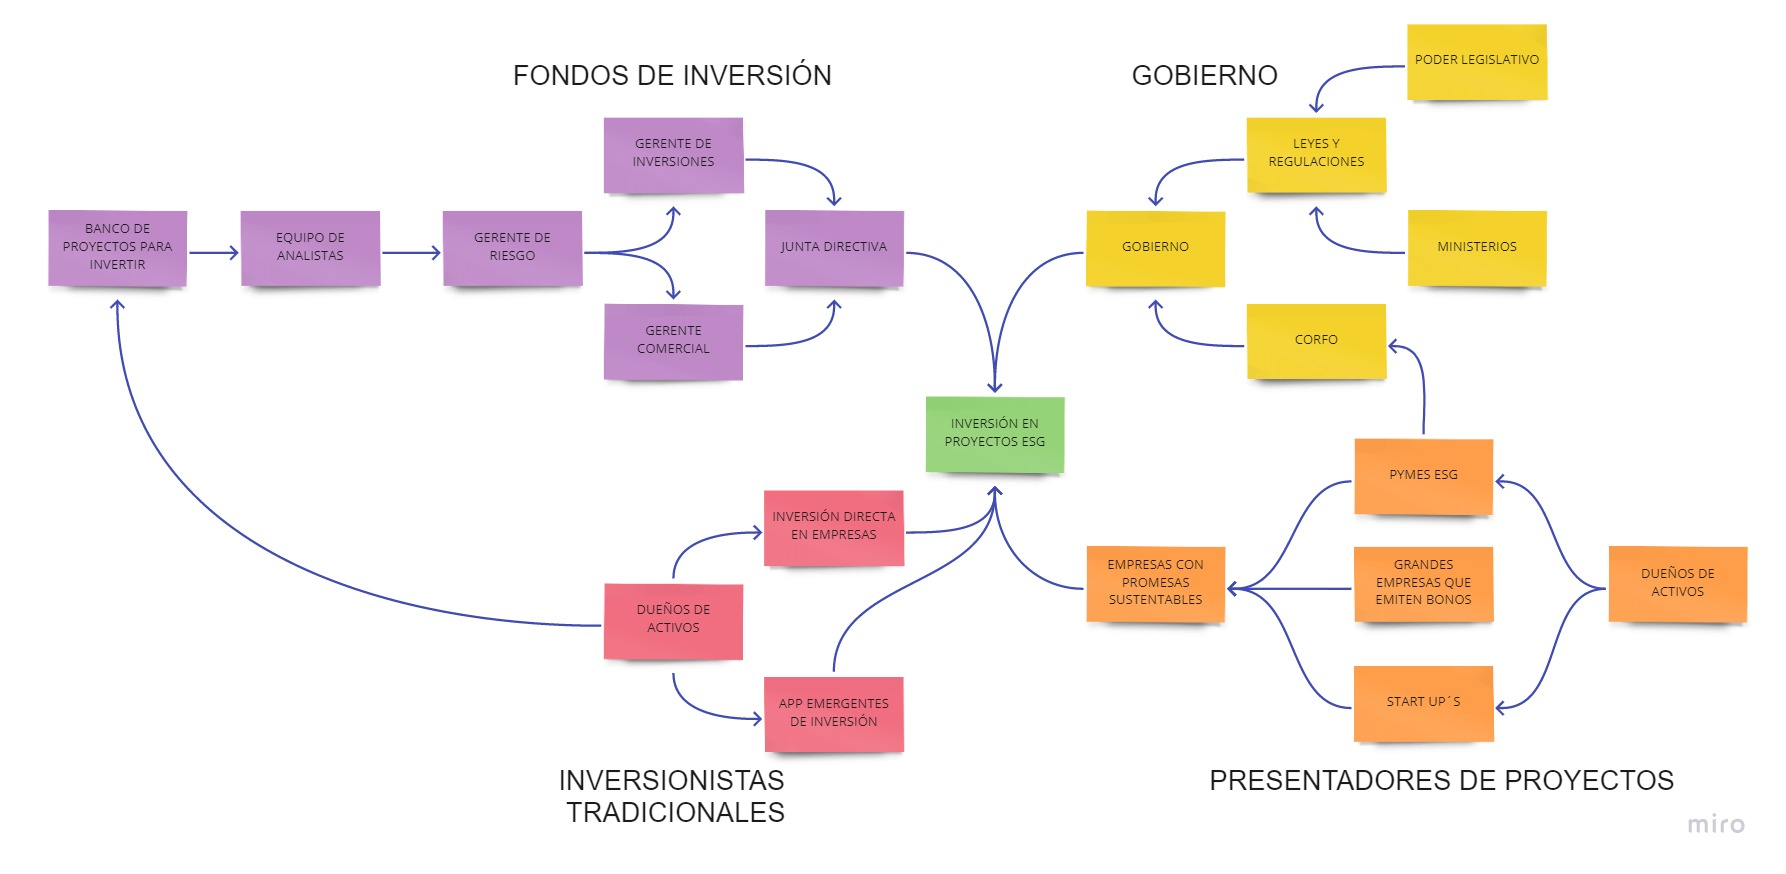
\includegraphics[scale=0.2]{Concept Map - Frame 1.jpg}
            \caption{Ecosistema ESG}
        \end{figure}
\end{itemize}

En este esquema, los actores pueden ser los inversionistas o dueños de activos que trabajan su capital de distintas formas. En rojo aparecen los inversionistas más "tradicionales", que depositan su dinero en aplicaciones modernas como Fintual o Racional. También, invierten a través de fondos de inversión, señalados en color morado, las cuales realizan contribuciones y compras de bonos en proyectos ESG.

En amarillo está el gobierno, que además de regular, también invierte con criterios ESG, y tiene instrumentos como CORFO. 

Finalmente, en Naranjo aparecen las empresas como tal, que tienen las ideas sustentables y que se desempeñan gracias a las inversiones.



\section{Entrevistas}

Según Belsom, Ahour, et all (2021), la interacción entre los dueños de activos y quienes los administran no siempre se condice, además de estar cada vez más presente las expectativas de las políticas ESG.

Por un lado, un incentivo para adoptar características ESG concuerda con los beneficios de la tasa de interés y puede depender del área geográfica donde se encuentran los actores, junto a las leyes y políticas públicas a las que se deben adecuar. 

Esta primera etapa de la investigación se centrará en los incentivos. La forma e importancia con que llegan los incentivos a todos quienes se involucran en la inversión de un proyecto es relevante para la toma de decisión. De este modo, las preguntas son variadas y diferentes dependiendo de las características del estatus del individuo.

\subsection{Preguntas:}

\begin{enumerate}
    \item ¿Qué entiende por Sustentabilidad? Es importante conocer las distintas respuestas, en este caso de forma muy general, con respecto al centro de la investigación.
    \item ¿Los retornos que espera en un proyecto sustentable son siempre de carácter monetario? Para este punto, conocer si los DM están esperando algo más allá de los beneficios monetarios comúnmente utilizados para evaluar cualquier proyecto. 
    \item ¿Qué tanto puede llegar a influir las características ESG en cuanto a los retornos por sobre las ganancias monetarias? Para unirla con la pregunta anterior, se espera que la mayoría indique que espera retornos en otros ámbitos.
    \item ¿Qué canales de información utilizan para medir características ESG?
    \item ¿Cuáles son las más influyentes?
    \item ¿Considera suficiente con cumplir planes regulatorios, o busca ir más allá en las apuestas con proyectos conscientes?
    \item ¿Cree que las políticas de estado están siendo suficientes, o espera que mejoren y aumenten en la línea sustentable?
    \item ¿Cómo enfrentar la crisis del calentamiento global con sus puestos de poder ante decisiones tan trascendentales?
    \item ¿Es la educación el proyecto más sustentable por el cuál las grandes empresas junto con el gobierno deberían apostar?
    \item ¿Piensa que una buena alternativa para inversiones ESG es basarse siempre en explicar bien los retornos monetarios, e incluirlos como eje principal para su desarrollo?
    
Estas preguntas desarrolladas de forma preliminar, están sujetas a cambio, pudiendo ser más, y dirigidas de forma distinta.

\section{Conslusiones}

En esta primera parte se estudió el experimento de Dean y Neligh (2019) en detalle, se explicó de forma simplificada el marco teórico y se conectó directamente con la investigación en inversiones sostenibles. 

Se espera que en los próximos pasos se puedan validar distintos puntos. El primero, es la hipótesis de que según el nivel en que se encuentre jerárquicamente el tomador de decisión, prestará atención a distintas métricas. Mientras que un analista observará los datos a detalle, centrándose en el dato más duro para evaluar un proyecto, el director de un fondo centrará su atención en el marco regulatorio y en los retornos más altos.

También, se presentó un esquema donde se mostraron todos los actores dentro del ecosistema ESG.


\vspace{3cm}


Nota (escala 1 a 7): 
\vspace{3cm}
Observaciones



\centering Firma Guía



    
\end{enumerate}





\newpage











































%ejemplo Plantilla



\end{document}
